\documentclass[beamer,crop,tikz]{standalone}

\usepackage{formation}
\definecolor{DarkBlue}{HTML}{003c72}
\definecolor{NormalBlue}{HTML}{0171c5}
\definecolor{LightBlue}{HTML}{01aef0}

\tikzset{textW/.style={
  text=white,
  align=center,
  }}

\begin{document}
  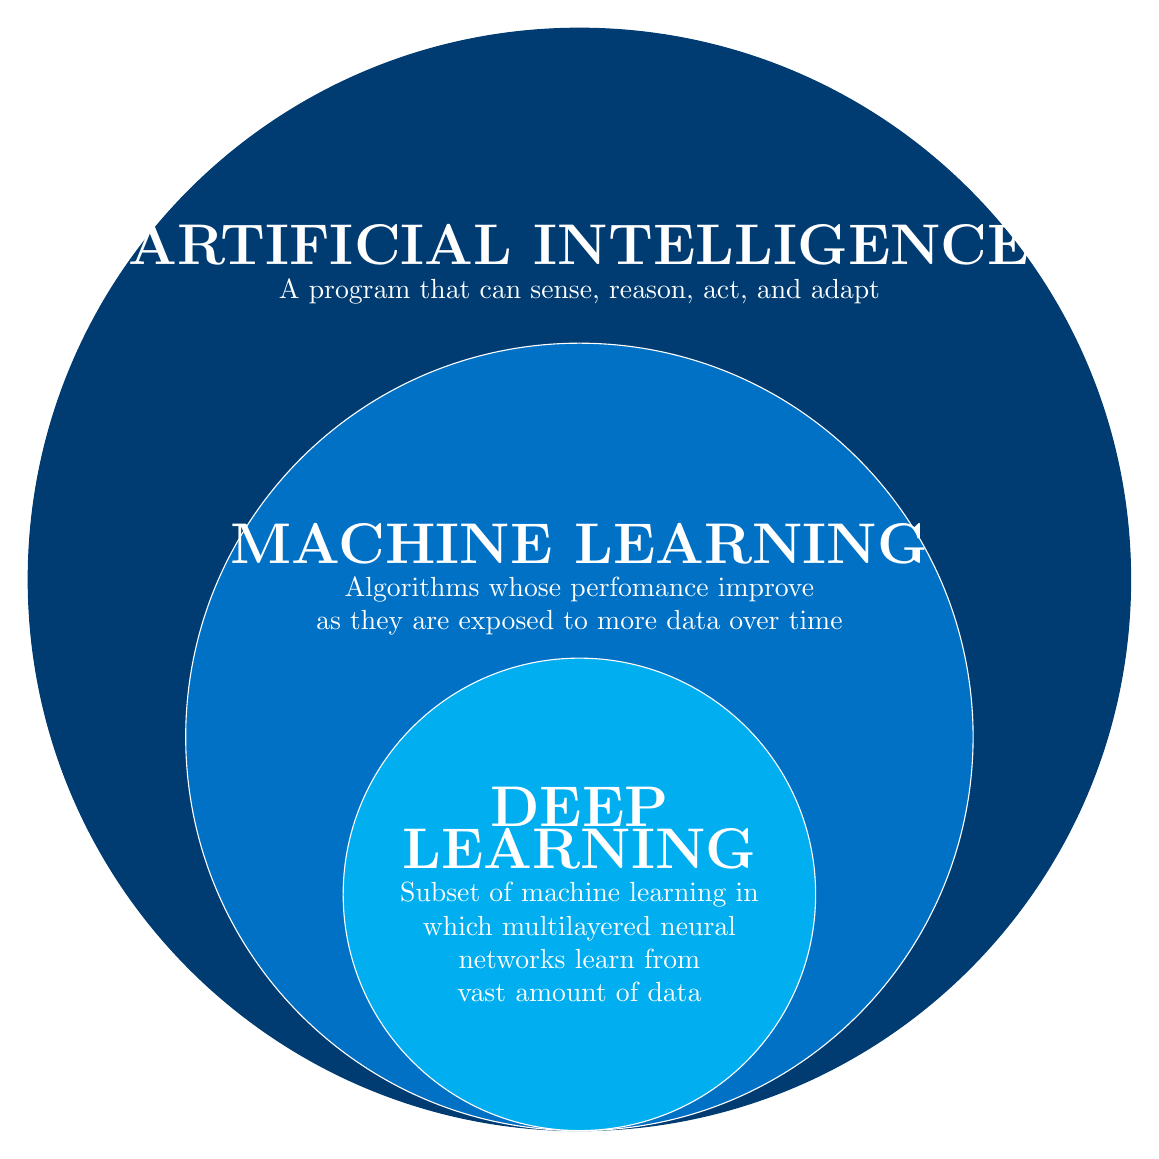
\begin{tikzpicture}
    \filldraw[DarkBlue] (0,6) circle (7); 
    \filldraw[NormalBlue,draw=white] (0,4) circle (5); 
    \filldraw[LightBlue,draw=white] (0,2) circle (3); 

    \node[textW] at (0,2) {\huge{\textbf{DEEP}}\\\huge{\textbf{LEARNING}}\\ Subset of machine learning in\\which multilayered neural\\networks learn from\\vast amount of data};
    \node[textW] at (0,6) {\huge{\textbf{MACHINE LEARNING}}\\
    Algorithms whose perfomance improve\\as they are exposed to more data over time};
    \node[textW] at (0,10) {\huge{\textbf{ARTIFICIAL INTELLIGENCE}}\\
    A program that can sense, reason, act, and adapt};
  \end{tikzpicture}
\end{document}

